\documentclass{article}
\usepackage[utf8]{inputenc}
\usepackage{setspace}
\usepackage{graphicx}
\usepackage{dirtree}
\usepackage[hang]{footmisc}
\usepackage{vhistory}
\renewcommand{\hangfootparskip}{10pt}
\setlength{\skip\footins}{1cm}
\setlength{\parskip}{1em}
\usepackage[a4paper, total={6in, 8in}]{geometry}


\title{%
Balancing Lustre Filesystem Resources strategies \\
\large Zenuity Oden Cluster (NGSC)}
\author{Carlos Thomaz - cthomaz@ddn.com}
\date{\today}
\begin{document}

\maketitle


\begin{center}
    
\includegraphics[scale=0.14]{logo.png}\\[1cm] 
\end{center}

\newpage

\begin{versionhistory}
    \vhEntry{Draft}{05.06.20}{CT}{Initial version}
    \vhEntry{v0.1}{05.09.20}{CT}{Initial version}
    \vhEntry{v0.2}{05.12.20}{CT}{Initial version}

\end{versionhistory}


\newpage
\section{Introduction}
This article describes high level strategies for managing and balancing high scale lustre file systems. Scalability is a key factor on distributed and parallel file systems. Such systems are usually measured and sized by performance (network throughput, sequential or random I/O workloads) and capacity. It is, of course, expected these two factors could grow over time.

With the highly adoption of parallel file systems by business oriented end-users, such as the crescent demand on Artificial Intelligence and Machine Learning data modeling, parallel file systems moved from solutions previously design as scratch data space towards a long term storage where performance, data resilience and availability is a requirement.

This article discusses strategies on managing and growing Lustre file system for long term projects where data distribution or maintenance may be required and what are the possible high level solutions and current challenges found addressing such problem.

\section{Problem Statement}
Unlike traditional High Performance Computing (HPC) deployments, business oriented projects often considers modular growth of resources over the time. System designers considers how a system may grow and how resources will be allocated over time obeying and satisfying the business Key Performance Indicators (KPIs) that includes cost of upgrades, system availability, performance requirements and others. 
When analysing the problem on storage stand point, some concerns are highlighted. Performance and capacity growth are obvious goals and reasons why an upgrade is planned. Availability is likely one of the biggest challenge and defies systems administrators to design a solution that won't impact, negatively, the business operation, guaranteeing the data availability and integrity during the upgrade process.

\subsection{Capacity growth}
As mentioned before capacity is one the reasons why an upgrade is required. Capacity on scalable and parallel file system grows adding additional storage devices (Lustre filesystem Object Storage Targets - OSTs). One or more OSTs can be added into an existing storage building block, sharing the same processing unit (Object Storage System) thus adding capacity but not necessarily additional performance.\footnote{Large systems OSS is often sized to provide its maximum bandwidth. Either disk storage back-end or network bandwidth is sized to be saturated providing the maximum efficiency.}
\subsection{Performance growth}
Storage performance can be measured in different ways. Bandwidth is usually an indicator for large sequential streams, while latency or IOPS\footnote{I/O Operations per Second} could be used to measure relatively small or atomic file level operations. When scaling performance, adding additional back-end storage device may not be enough. If the system controller (MDS or OSS) was sized to utilize efficiently the entire bandwidth, the addition of back-end storage (any type of media) will only help to grow capacity.

The opposite may be also true. Hypothetically speaking, increasing the network or memory bandwidth may not be enough to decrease high disk latency neither increase bandwidth since the bottleneck may be the disk device itself or other limitations such as memory latency, lack of CPU resources managing too many threads, network latency.
These cases usually requires addition of entire building blocks, on Lustre file system vocabulary, Object Storage Servers or Metadata Storage Servers, referring to the set of servers and disk storage. 
By design, Zenuity ODEN cluster will always grow by adding atomic building blocks, with a predefined configuration which is identical to the initial setup.

\subsection{ODEN's storage building blocks}
ODEN cluster compromises a total of 6 so called \textit{Firezones}. Firezones are a set of computational resources (Servers, GPUs, network and storage) that are self contained and independent. These Firezones will be accessible by users submitting jobs and running different workloads. Each firezone owns two filesystem namespaces that are independent from each other. These two namespaces are designed to provide higher data availability splitting the storage into two independent failure domains and reducing the chances of a hardware or software failure to impact access to the parallel filesystem.

Each filesystem has been designed without single point of failure, where components are redundant and hard disk devices and SSDs are protected by multiple redundancy layers potentially allowing multiple simultaneous failures without loosing access to data. The filesystem is composed by Highly available building block pairs serving different functions (Metadata Storage Systems and Object Storage Systems layers\footnote{Two type of OSS building blocks has been designed: Flash layer OSS and HDD Layer OSS}).


\subsubsection{Metadata Storage Systems}
A total of two MDS pairs will be configured on each namespace. Each MDS pair will provide two Metadata Targets (MDT) with enough i-node allocation for the entire file system lifecycle and a possibility to configure DOM\footnote{Data On Metadata}. 

The MDSs and MDTs are not supposedly to grow and upgrade procedures are not required for these building blocks.

\subsubsection{Object Storage Systems}
One namespace will be initially configured with five OSS building blocks, being two of them a Flash layer OSS and three of them HDD layer OSS. Each HDD based OSS provides 50GiB/sec of sustained sequential throughput and usable capacity of 5PiB. The Flash layer OSS are inteded to use with relatively small I/O workloads. The namespace is subjected to upgrades when additional capacity or performance is required. 


\subsection{Lustre File System - OST allocation algorithm}
To optimize file system performance, Lustre MDT assigns file stripes to OSTs based on two allocation algorithms. Round-robin allocator give preference to location (spreading out stripes across OSTs to increase network bandwidth utilization) and the weighted allocator gives preference to available space (balancing loads across OSTs). Threshold and weighting factors for these two algorithms can be adjusted by the user. The MDT reserves 0.1 percent of total OST space and 32 inodes for each OST. The MDT stops object allocation for the OST if available space is less than reserved or the OST has fewer than 32 free inodes. The MDT starts object allocation when available space is twice as big as the reserved space and the OST has more than 64 free inodes. Note, clients could append files no matter what object allocation state is.\footnote{Definition extracted from Lustre 2.12.x manual}

One namespace or filesystem is composed by multiple OSTs. Oden cluster's design considers a total of 26 OSTs being 8 of them based on NVMe Flash storage and 18 OSTs based on rotational devices (Hard Disk Drives - HDD). These OSTs are hosted by multiple OSS embedded virtual machines managed by the DDN SFA storage appliances. 
The current design for an initial deployment will follow the schema on table \ref{tab:ost-allocation}.
\begin{table}[h]
\centering
 \begin{tabular}{||c c c c c||} 
 \hline
 Layer & Storage Block & OST indexes & Capacity & Est. Performance per OST\\ [0.5ex] 
 \hline\hline
 Flash & NV400[1] & [0-3] & N TiB & xxGiB/sec \\ 
 \hline
 Flash & NV400[2] & [4-7] & N TiB & xxGiB/sec \\ 
 \hline
 HDD & ES7990[1] & [8-13] & N TiB & xxGiB/sec \\
 \hline
 HDD & ES7990[2] & [14-19] & N TiB & xxGiB/sec \\
 \hline
 HDD & ES7990[3] & [20-25] & N TiB & xxGiB/sec \\
 \hline
 All & NV400/ES7990 & [0-25] & N TiB & xxGiB/sec \\ [1ex] 
 \hline
\end{tabular}
\caption{Initial OST allocation and details per namespace}
\label{tab:ost-allocation}
\end{table}

\subsubsection{OST pools}
For projects designed with hybrid OSTs (flash and Hard Disk) is encouraging to configure Lustre OST pools. OST Pools will provide a resource division and may help prevent wrong utilization of different type of medias. If not defined, Lustre will distribute data across all the OSTs regardless its type. The OST allocator won't differ the media technology or different specifications without an implicit utilization of OST pools, reason why it is strongly recommended to design the OST pool hierarchy before production.

At least, two OST pools shall be created to avoid miss-utilization of resources: flash.pool and hdd.pool. These two OST pools are sub-sets of the entire namespace (Table \ref{tab:ost-pools}).

\begin{table}[h]
\centering
 \begin{tabular}{||c c c c||} 
 \hline
 OST pool & Media type & OSSs & Storage Controller type \\ [0.5ex] 
 \hline\hline
 flash.pool & NVMe & [0-3] & ES400NVX \\ 
 \hline
 hdd.pool & Rotational device & [4-21] & ES7990X\\
 \hline
 \end{tabular}
 \caption{Tiers - Hybrid namespace}
 \label{tab:ost-pools}
\end{table}

Additionally, table \ref{tab:example-ost-pools} shows OST pools that could be created to enable finer grain data distribution. It is important to keep in mind that too many OST pools may create challenges managing data, so it is recommended to do not over-utilize such resource to prevent higher data management complexity.

\begin{table}[h]
\centering
 \begin{tabular}{||c c c c||} 
 \hline
 OST pool & Media type & OSSs & Storage Controller type \\ [0.5ex] 
 \hline\hline
 flash.nv1 & NVMe & [0-1] & ES400NVX \\ 
 \hline
  flash.nv2 & NVMe & [2-3] & ES400NVX \\ 
 \hline
 hdd.es7990-1 & Rotational device & [4-9] & ES7990X\\
 \hline
  hdd.es7990-2 & Rotational device & [10-15] & ES7990X\\
 \hline
  hdd.es7990-3 & Rotational device & [16-21] & ES7990X\\
 \hline
 \end{tabular}
 \caption{Example of OST pools}
 \label{tab:example-ost-pools}
\end{table}

Distinct OST pools per SFA appliance may be helpful when managing data and measuring performance. Measuring
building block performance is often desired and may require an easy workload generation that only actuates on targets in a specific appliance. Having an OST pre-defined will help to assign a specific target directory or file to one specific set of OSTs. This could be done with a single command, as long as the OST pool is created.

    \begin{verbatim}
    # lfs setstripe <filename|dirname> --pool|-p pool-name
    \end{verbatim}
Utilization of OST pools become mandatory when data re-balancing and fine grain data manipulation and  data placement is required. 

\section{Zenuity Oden's parallel File System strategies}
Based on previous meetings and technical conversations between DDN and HPE, data re-balancing and management for Oden cluster may not be required in its full capability. It is expected each namespace to grow up several times, resulting in potential larger usable capacity file system and larger aggregate peak performance per namespace. However, one possible strategy is to implement a \textit{Fill up and Append} policy. This may work under certain scenarios. 

The full re-balancing is not encouraging for systems with capacity on that magnitude. At least not without special tools and \textit{Data-loss mitigation} strategy, not mentioning an extended period of time where the file system will be required to be put in maintenance mode. A \textit{Partial re-balancing} may be needed for maximum utilization of resources.

\subsection{Full Data Re-balancing}
The idea of data re-balancing is to distribute the existing data residing on previously deployed OST across the recently added resources, in a way that, after the data re-balancing is done, all OSTs are evenly used. In this scenario we assume no new data will be ingested into the file system until re-balancing is completed (\ref{fig:full-rebalance strategy}. 


\begin{figure}[h]
    \centering
    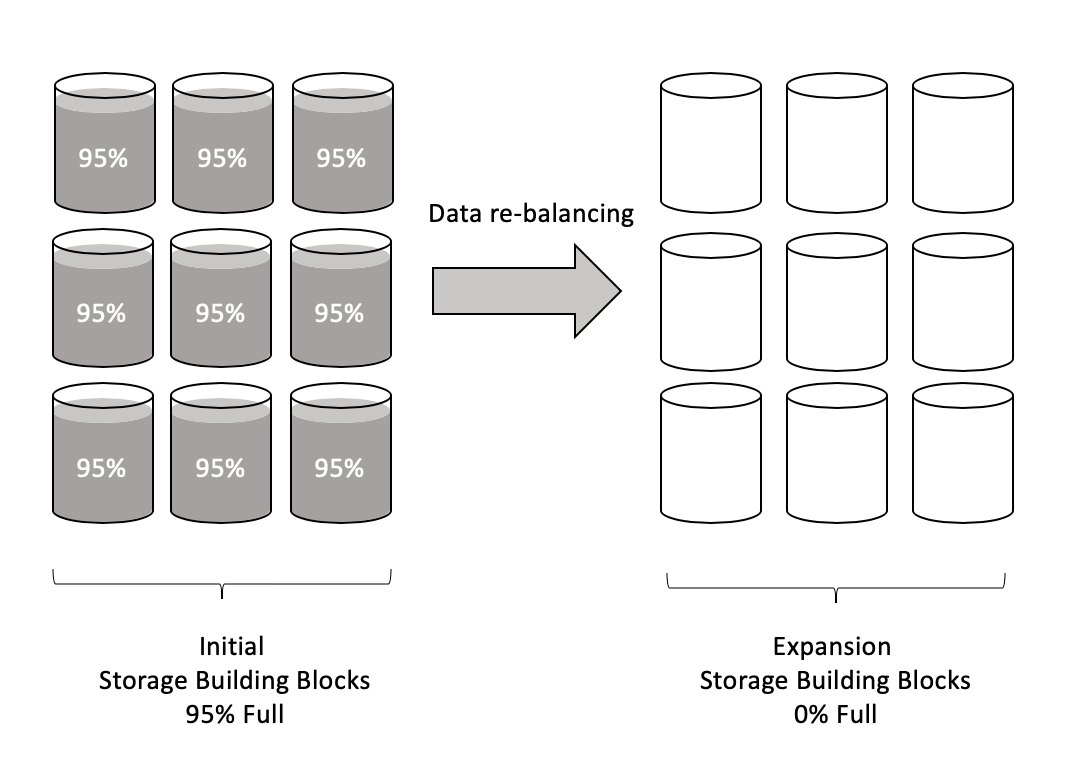
\includegraphics[scale=0.37]{full-rebalance.png}\\[0.5cm] 
    \caption{Addition of $N (9)$ OSTs and Data re-balancing}
    \label{fig:full-rebalance strategy}
\end{figure}


This operation is extremely expensive in terms of required time and resources. Some of the challenges, but not limited to, are: 
\begin{itemize}
    \item Heavy MDT and OST scanning and I/O overhead
    \item Lack of parallelism when using standard tool set. Long maintenance window
    \item Risk of data loss
\end{itemize}

\subsubsection{MDT and OST overhead}
Although this strategy is theoretically possible (Lustre even provide basic tools to perform such migrations) on large scale systems is proven to be unsuccessful. One of the observed side effects of moving a such amount of data is  MDS/MDTs overloading and the increased latency to access attributes (file size) that are stored on OSTs. Applying this strategy requires a check or comparison of every file resulting in a large array of atomic operations until the object is re-balanced. Depending on the effectiveness of tools being used, as well the methodology to calculate and take decision about balancing the data across new OSTs, this mechanism becomes very slow.

\subsubsection{Lack of parallelism when using standard tool set}
Lustre has no internal mechanisms that transfer data from OSTs transparently. Instead, it relies on utilization of \textit{copy tools} that has been modified to understand Lustre file semantics such as extended attributes. 
Typically the Lustre community relies on copy tools such as lustre\_rsync or \textit{lfs migrate}. The major issue are the serialized approach that isn't suitable for large data transfers.

\subsubsection{Risk of data loss}
Manipulating huge amount of data is always subjected to the risk of data being lost or corrupted. Running these mechanisms for large periods may increase the risk of external factors to contribute for a possible data corruption. For example, a temporary network failure may induce errors that needs to be well understood and captured by the data movement scripts, otherwise it may cause data corruption. To guarantee data integrity file level based data movement may also require to keep the original file until is absolutely confirmed the data has been copied and is identical, causing a temporary space overhead as well duplicate i-node allocation.

\subsubsection{Advantages of this method}
The advantage of this method, assuming it will work, is a file system well distributed where end-users may not need too much attention to where to store their files since all OSTs will provide the same capacity. 
In this scenario, there's a potential bandwidth increase, specifically for writes workload, because files could be now  written across all available disks ($N$), instead of only new disks ($N/2$). In this case the OST allocator will have no problems distributing the data across all available targets.

\begin{figure}[ht]
    \centering
    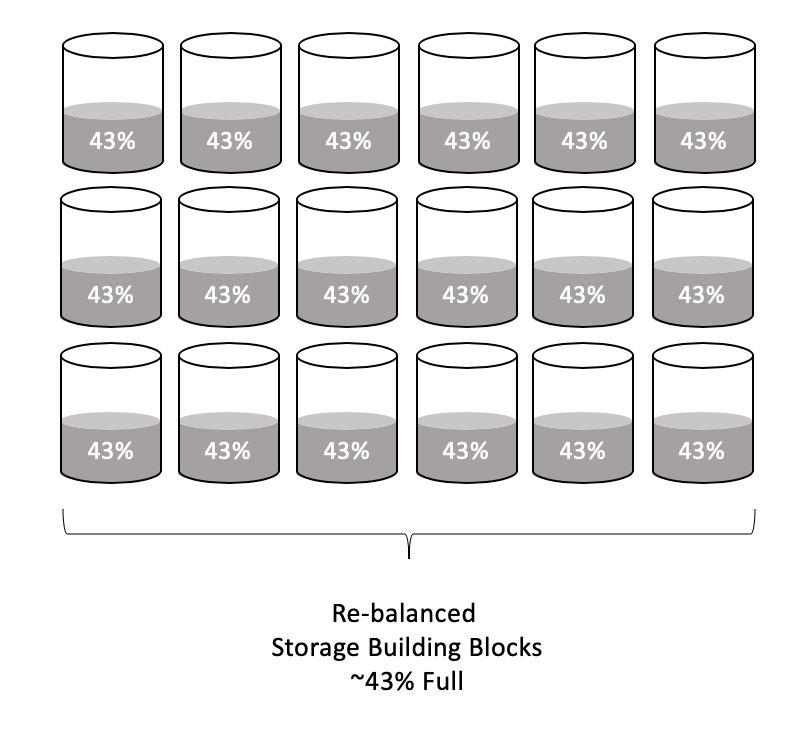
\includegraphics[scale=0.37]{OSTs-rebalanced.png}\\[0.5cm]
    \caption{OSTs re-balanced and usable capacity evenly distributed $N(18)$}
    \label{fig:re-balanced OSTs}
\end{figure}


\subsection{Fill Up and Append}
This strategy is a lot easier and faster, and more realistic. It allows to add new storage building blocks and make it available for use almost immediately after. Since it doesn't requires data re-balancing the additional capacity will be promptly available for users (figure \ref{fig:fillup}). However, this strategy relies on a more detailed and efficient storage management as well a  disciplined usage of Lustre OST pools and other resources. 
Ideally at least one OST pool should be created when the filesystem is initially deployed. The upgraded OST set would be added to a second OST pool, so once in production new data should be always be written to the second OST pool avoiding possible errors (\textbf{ENOSPC}) when trying to write in a full or almost full OST. 

\begin{figure}[h]
    \centering
    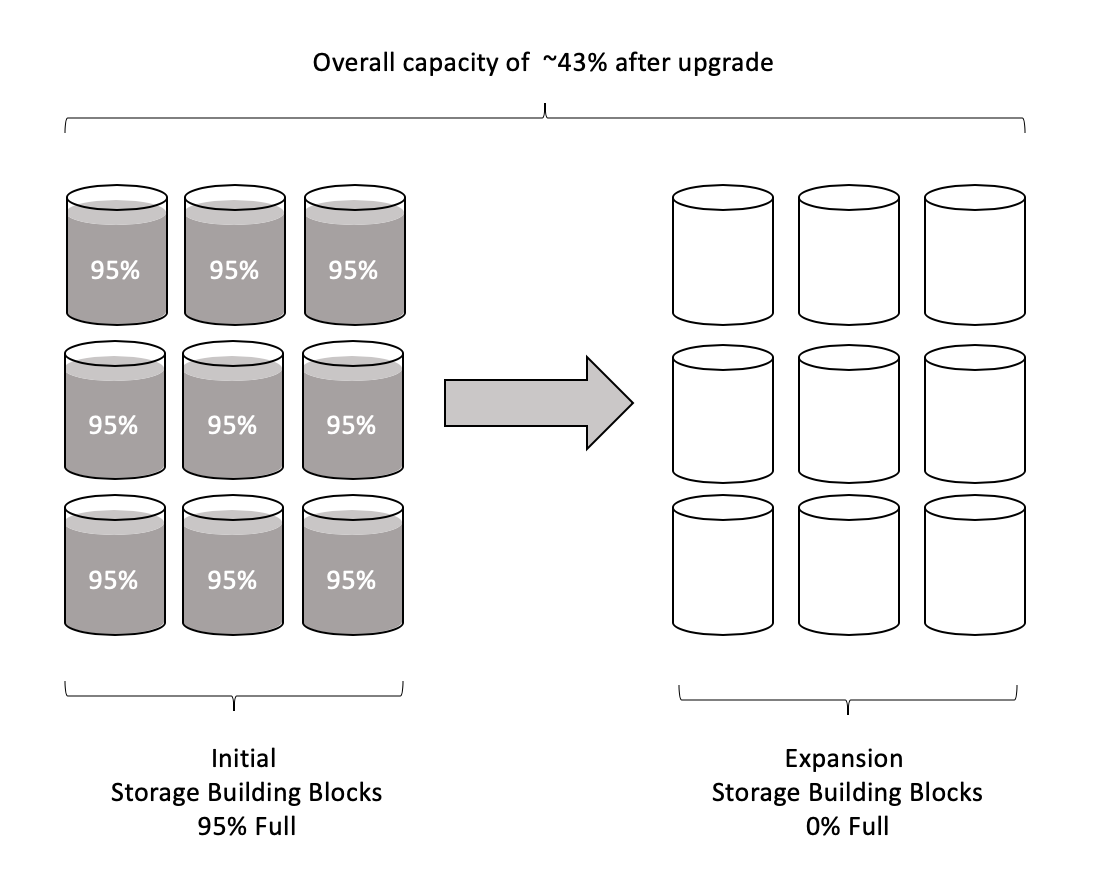
\includegraphics[scale=0.39]{fillup-append.png}
    \caption{Writable OSTs after upgrading equals to $N(9)$}
    \label{fig:fillup}
\end{figure}

To mitigate problems, OSTs that belongs to the first pool could be \textit{deactivate} on the MDS, meaning the OST will be no longer available for writing, or no new objects will be allocated on these OSTs, but remove and modify files that resides on these OSTs will still be possible. 

This strategy, as mentioned before, must be aligned with the high level directory structure. For instance, the allocation of directories and sub-directories should be designed previously having in mind the possibility of upgrading the system and adding new storage devices in the future. 

According to the table \ref{tab:ost-pools} a possible directory hierarchy could be designed as follow

\dirtree{%
.1 /lustre.
.2 datasets\DTcomment{Important Data files}.
.3 data1.
.2 home\DTcomment{Home directories}.
.2 scratch\DTcomment{Scratch files}.
.2 nvme\DTcomment{NVME storage tier}.
}    

In principle the NVMe based flash tier should be used only for small files and heavy random I/Os. Usually a quota enforced \$HOME directory is also configured on the flash layer (when not configured outside the parallel file system).

\dirtree{%
.1 /lustre.
.2 datasets.
.3 data1\DTcomment{OST pool: hdd.pool}.
.2 home\DTcomment{OST pool: flash.pool}.
.2 scratch\DTcomment{OST Pool: hdd.pool}.
.2 nvme\DTcomment{OST pool: flash.pool}.
}    

Notice this strategy may cause future problems when, for example, an upgrade is requested. Ideally the OST pools should be enumerated or labeled accordingly. For instance a fine grained OST pool design (table \ref{tab:example-ost-pools}) could be a better option if implemented additionally to table \ref{tab:ost-pools}.

\dirtree{%
.1 /lustre.
.2 datasets.
.3 data1\DTcomment{OST pool: hdd.pool}.
.2 home\DTcomment{OST pool: flash.nv1}.
.2 scratch\DTcomment{OST Pool: hdd.es7990-1}.
.2 nvme\DTcomment{OST pool: flash.pool}.
}    

Then, in case of an upgrade (for example, additional 3 DDN ES7990X appliances) additional OST pools should be also created and made available.
\begin{table}[h]
\centering
 \begin{tabular}{||c c c c||} 
 \hline
 OST pool & Media type & OSSs & Storage Controller type \\ [0.5ex] 
 \hline\hline
 flash.nv1 & NVMe & [0-1] & ES400NVX \\ 
 \hline
  flash.nv2 & NVMe & [2-3] & ES400NVX \\ 
 \hline
 hdd.es7990-1 & Rotational device & [4-9] & ES7990X\\
 \hline
  hdd.es7990-2 & Rotational device & [10-15] & ES7990X\\
 \hline
  hdd.es7990-3 & Rotational device & [16-21] & ES7990X\\
 \hline
  hdd.es7990-4 & Rotational device & [22-27] & ES7990X\\
 \hline
 hdd.es7990-5 & Rotational device & [28-33] & ES7990X\\
 \hline
 hdd.es7990-6 & Rotational device & [34-39] & ES7990X\\
 \hline
 hdd.pool-2 & Rotational device & [22-39] & ES7990X\\
 \hline
 \end{tabular}
 \caption{Additional OST pools after upgrade}
 \label{tab:example-ost-pools-upgrade}
\end{table}


With the additional OSTs and OST pools deployed, a directory structure should then look like:

\dirtree{%
.1 /.
.2 datasets.
.3 data1\DTcomment{OST pool: hdd.pool}.
.3 data2\DTcomment{OST pool: hdd.pool-2}.
.2 home\DTcomment{OST pool: flash.nv1}.
.2 scratch\DTcomment{OST Pool: hdd.es7990-4}.
.2 nvme\DTcomment{OST pool: flash.pool}.
}    

Notice this directory structure is a simple example. Obviously a production file system has a more complex structure with deeper trees and other dependencies. The main focus is on the utilization of rotational devices pools. In this example, after de-activating the full OSTs is then necessary to re-apply new \textit{Lustre striping} settings pointing directories to the second recently created pool named as \textit{hdd.pool-2}. 

\subsubsection{File Layouts}
In conjunction with the OST pool policy, \textit{Progressive File Layout} should be used enforcing new files to be spread out over the newly added OSTs optimally. PFL intends to simplify the use of Lustre so that users can expect reasonable performance for a variety of normal file IO patterns without the need to explicitly understand file placement nor IO model or Lustre usage details in advance. In particular, users do not necessarily need to know the size or concurrency of output files in advance of their creation and explicitly specify an optimal layout for each file in order to achieve good performance, for both highly concurrent shared-single-large-file IO or parallel IO to many smaller per-process files. Combining PFL with OST pools will simplify the data management tasks for end users as well systems administrators. 

For instance, adopting the Fill Up and Append model, the PFL would be unique for the entire filesystem lifecycle. Assuming the increments will have the same number of OSTs, PFL could be universal for the entire file system, assuming for example a maximum of 18 components per upgrade cycle. 


\subsubsection{Performance considerations}
It is important to notice that \textbf{Write} performance will be affected in this utilization model. Unlikely the full re-balanced model where the total $N$ OSTs would be available for write, in this model only $N/2$ would. The initial OSTs would be de-activated thus only aggregating performance on \textbf{Reads}. 

For \textbf{Acceptance} criteria reasons and \textbf{KPI matching metrics}, the performance of a namespace must be assumed as the sum of initial and partial performance metrics. For instance, the maximum capacity and theoretical performance of a single namespace 5PiB and 200GB/sec (peak sequential throughput). The initial namespace deployment will measure through standard benchmarks and workloads (explained in details on the Acceptance procedures and Operational procedures document). Upgrades will be measured isolated (before being integrated into the live filesystem) and the proportional peak performance will be summed to the initial performance benchmark numbers. Capacity is also subjected to be increased non-linearly, due the new capacity HDD models that may become available during the lifecycle of this project. Performance will always be respected according to the models that will impose the number of required HDDs (in case of capacity change - Assuming HDDs with the same capacity will be available during the course of the project, then the same number of drives will be delivered per update cycle). 

\subsection{Partial data migration}
Partial data migration, in the context of this project, is not intended to re-balance the entire filesystem after an upgrade. This technique may be necessary in some use-cases where minor data sets will need to be moved or duplicated. Data residing on the de-activated OSTs may be required to be moved or replicated (mostly because the data is subjected to changes). In these scenarios, there is no option other than partial data migration.

The data migration consists of a set of processes that combined provides a solid and fast mechanism to migrate data between file systems or within a file system. In general terms the steps consists of:
\begin{enumerate}
    \item Generate a list of files to be migrated (Delta detection)
    \item Configuration and job distribution
    \item Data verification and purging
\end{enumerate}

\subsubsection{Delta Detection}
Delta detection will tell what are the files to be migrated provided a certain scope (e.g.: file attributes like size, mtime, UID, GID, etc). It does require efficient resource allocation and smart algorithms that maximize performance. For very small data sets tools like lustre\_rsync bundles up the delta detection. However, for large amount of data, it is necesary to decouple and be able to run delta detection in parallel. 

One option available today is the utilization of MPI based file utilities, more specifically DCMP. DCMP is a MPI program that compare files recursively with same relative paths within two different directories. DCMP can be configured to compare a number of different file properties. 

\subsubsection{Configuration and job distribution}
Once the list of files to be migrated is created a set of jobs needs to be configured and submitted. Just like the Delta detection, the job distribution in very simple cases is bundled up into the program that will control the data manipulation, as an example of lustre\_rsync. However, to make it scale is necessary to use different methods where two issues must be addressed: 
\begin{itemize}
    \item Millions of small files
    \item Parallelism for very large files
\end{itemize}

Ability to launch several jobs in parallel that won't interfere with each other is important and could be achieved with smart scp or equivalent \textit{Lustre aware} copy commands. 
The parallelism for one or multiple very large files must be also addressed so multiple threads or MPI ranks reads a file extent (or chunk), transfer to the destination and write it. Similarly to DMCP, DCP is a MPI copy tool that allows multiple MPI process to effectively copy regions of a file parallelizing the access and copy of one very large file. It also works for several small files where the number of simultaneous threads are more important than a single file operation.

\subsubsection{Data verification and purging}
Once the files are copied, it may be necessary to certify its integrity and deletion of original one. This phase also includes Lustre changelog cleanup and possibly layout manipulation (depending on the strategy). 

\subsubsection{Considerations for Partial Data Migration}
Partial Data migration will be inevitable at some point. Either for backup purposes, data duplication or similar tasks. For very large file system is highly recommended to have dedicated resources or at least resources that could be used without interruption for several hours (data movers). 

Another important consideration is the impact of DCMP and DCP on metadata. Increasing the number of MPI ranks to accelerate the data migration is tempting, but it may cause Metadata processing shortage which may be unacceptable for a file system in production.

Throttling I/O resources is an important tool to be considered. Either through a controlled number of MPI jobs (in case of MPI File Utils) or through a Lustre QOS (limiting the number of RPC for a given user authorized to perform data migration). 

Specially when moving data within a file system the method can add a significant large overhead to copy the objects from Lustre servers, all the way to the client layer and put it back potentially into the same set of servers but in different path. Ideally this should be implemented on the server side where data is transferred from OSTs to OSTs transparently. A project addressing such scenario still under development at DDN called \textit{ldmigrate}. Ldmigrate aims to move the object data from source OSTs to destination OSTs but maintaining the Metadata information. This tool will replace the DCP when moving data within the same namespace saving client resources (won't require client processing) and adding an implicit approach.

Ultimately, there are other solutions that could be used for partial data migration that includes DDN Stratagem, HPE DMF or open source choices such as Robinhood in conjunction with handful number of copy tools. These solutions mostly address the Policy management layer (what and when it needs to be moved/copied), as well some minimal reports. However, it adds a layer of complexity that require specific management and eventually assume particular tasks that must be well understood, such as the impacts of high performance scans on a \textit{live} file system. 

\subsubsection{Large Files Use Case}
One possible and likely scenario is the design of methods for large file migrations. This would affect only large files and possibly pre-defined subdirectories where it's known to store large files mostly accessible for Reads (WORM mostly). In this scenario the data transfer is mostly network bound  and is less disruptive in terms of performance impacts on the file system. Assuming the path of files are known, as well the destination poo, this migration could be invoked using Lustre File Level Redundancy. 
Consider the following directory structure.

\dirtree{%
.1 /lustrefs.
.2 datasets.
.3 data1\DTcomment{OST pool: hdd.pool}.
.4 very-large-files.
.3 data2\DTcomment{OST pool: hdd.pool-2}.
.2 home\DTcomment{OST pool: flash.nv1}.
.2 scratch\DTcomment{OST Pool: hdd.es7990-4}.
.2 nvme\DTcomment{OST pool: flash.pool}.
}    

The files on /lustrefs/datasets/very-large-files/ directory inherited the OST pool definition from its parent directory, thus Lustre Objects resides on OSTs that belongs to hdd.pool.

In case of need to free space on hdd.pool would be possible to invoke a file replication and after completed a mirror deletion. This is not a single step process, but could be reasonably automated with \textit{lfs mirror} commands.

Alternatively, the file could be implicitly copy from, for example, /lustrefs/datasets/very-large-files/ to /lustrefs/datasets/data2/some-sub-dir using the mentioned before copy tools. 

The disadvantage of this method is mix directory structure with different set of OST pools. As mentioned before, for better organization, a certain parent directory should contain only subdirectories that inherited the same OST pool. Using the FLR approach may mix this up becoming inconvenient to manage. 

\section{Conclusions}
Avoiding massive data re-balancing is recommended for large file systems. Fill Up and Append method in conjunction with Lustre Progressive File Layout (PFL) provides a mid term solution that address capacity, performance and data management challenges.

Partial data migration may be required during the filesystem life cycle. When it so, it is recommended to have computational resources ready to execute such explicit tasks, since Lustre doesn't provide yet a transparent mechanism for data movement. These jobs will require job scheduling integration and possibly very specifics queue definitions and user's permission. It is also recommended further investigation on Job placement policies as well implementation of job dependency (job chaining) to guarantee that data manipulation workflow is executed accordingly preventing data loss or resources starvation or over-utilization. 

Lustre QOS may be used to limit the number of Lustre RPC per user, so throttling performance and avoiding too much metadata pressure that may impact the Service Level Agreement required for production. 

A fully automated solution will also require a policy engine that may trigger tasks automatically. Policy Engine is out of scope at this moment. 

Finally a review and agreement of how to measure performance to match the KPI for each namespace must be agreed since the execution of benchmarks on a live system will impact the production and it is not recommended. Also, depending on the strategy adopted it may not be technically possible to run end-to-end benchmarks thus requiring assumptions about how to calculate overall system peak performance.

\end{document}